% !Mode:: "TeX:UTF-8"
% !TEX root = ..\Literature_Translation.tex
\chapter{案例分析}
\section{遗传算法在多品种装配生产排序中的应用}
\subsection{背景简述}
在中小型装配生产企业的生产实践中,由于产品品种的变动使得某些工作站或工位需要更换工装,包括更换夹具和辅具,其更换操作时间有的只有半分钟,而有的却要十几分钟,一般在1 -- 2分钟左右。然而,品种变动经常引起多个工作站需要更换工艺装备,这样总工艺辅助时间可能达到l0 分钟甚至几十分钟以上,品种变动次数增多以后,总工艺辅助时间的增加对装配生产的影响是不能忽视的。

为方便分析研究,符号说明如下:

\begin{tabular}{ll}
$i$ & 产品品种,$i = 1,2,...,n$\\
$M_k$ & 工作站,其中$k = 1,2,..,m$\\
$(i,j,M_k)$ & 在工作站$M_k$上,加工的产品由品种$i$改变为品种$j$时引起的辅助时间需求。\\
$d(i,j)$ & 品种$i$直接排在品种$j$前面装配时各工作站的工艺辅助时间需求总和。
\end{tabular}

可以得到:
\begin{equation}
d(i,j) = \sum_{k=1}^m (i,j,M_k) \label{equ:3}
\end{equation}

同样,可以得到一个工艺辅助时间需求矩阵:
\begin{equation}
D = \begin{pmatrix}
d(1,1) & d(1,2) & \cdots & d(1,n)\\
d(2,1) & d(2,2) & \cdots & d(2,n)\\
\vdots & \vdots & \ddots & \vdots\\
d(n,1) & d(n,2) & \cdots & d(n,n)
\end{pmatrix}
\end{equation}

易知$d(i,j) \neq d(j,i)$,设$n$维向量表示一个品种安排顺序$X = \{x_1,x_2,...,x_n\}$,这样,由于品种的更换而产生的总工艺辅助时间可以表示为:
\begin{equation}
T = \sum_{i = 1}^{n-1} d(x_i,d_{i+1})
\end{equation}
式中$x_i \in \{1,2,...,n\}, i = 1,2,...,n$。设在制品装配序列的最后一个产品品种为$p$,则该问题的数学模型为:
\begin{equation}
\begin{cases}
\min \  f(x) = d(p,x_1) + \displaystyle\sum_{i = 1}^{n-1} d(x_i,x_{i+1})\\
s.t.\ : D\ is\ given
\end{cases}
\end{equation}
可以将多品种装配顺序的安排问题看作商旅问题(TSP)。

某小型企业,有装配线一条,生产12种不同类型的产品,根据\eqref{equ:3}求得
工艺辅助时间需求矩阵,如\eqref{equ:4}所示。
\begin{equation}
D =\quad \bordermatrix{
	~ & 1 & 2 & 3 & 4 & 5 & 6 & 7 & 8 & 9 & 10 & 11 & 12\cr
	1 & 0 & 11 & 6.1 & 6.2 & 7.4 & 7.4 & 5.1 & 6.2 & 4.5 & 12.5 & 11.6 & 9.3\cr
	2 & 6.5 & 0 & 7.1 & 5.2 & 6.2 & 6.2 & 5.3 & 7 & 4.3 & 5.2 & 10 & 9.5\cr
	3 & 4.3 & 4.3 & 0 & 5 & 3.7 & 3.7 & 4.3 & 5.1 & 4.2 & 6.2 & 6.1 & 5.5\cr
	4 & 4.2 & 4.2 & 3.2 & 0 & 5.9 & 5.9 & 5.3 & 4.7 & 4.3 & 5.1 & 7.4 & 5.1\cr
	5 & 7.8 & 6.1 & 8.4 & 4.4 & 0 & 0 & 11.2 & 9.2 & 8.5 & 11.4 & 7.3 & 13.3\cr
	6 & 7.8 & 6.1 & 8.4 & 4.4 & 0 & 0 & 11.2 & 9.2 & 8.5 & 11.4 & 7.3 & 13.3\cr
	7 & 4.9 & 4.3 & 6.5 & 5.7 & 10.5 & 10.5 & 0 & 4.5 & 3.7 & 11.3 & 4.5 & 8.9\cr
	8 & 13.5 & 11 & 13 & 6.8 & 13.4 & 13.4 & 3.8 & 0 & 11.3 & 9.5 & 9.7 & 9.7 \cr
	9 & 13.6 & 7.7 & 11 & 7.3 & 12.5 & 12.5 & 6.7 & 7.5 & 0 & 13.1 & 8.4 & 7.3\cr
	10 & 9.3 & 6.9 & 7.7 & 7.9 & 1.5 & 1.5 & 8.3 & 6.7 & 7.5 & 0 & 11.3 & 10.3\cr
	11 & 7.5 & 5.3 & 4.3 & 9.5 & 6.5 & 6.5 & 7.5 & 5.5 & 11.7 & 5.7 & 0 & 9.6\cr
	12 & 5.8 & 7.3 & 5.4 & 4.7 & 7.6 & 7.6 & 8.9 & 8.7 & 11.5 & 5.3 & 11.6 & 0 
}\label{equ:4}
\end{equation}
\subsection{算法步骤及实现}
用遗传算法求解TSP问题是一种实用有效的方法,其采用一种基于自然选择和群体遗传机理的搜索算法,对于复杂问题通过选择、交叉、变异等遗传操作寻找到优化的解。记$N(p)$为种群大小,$P(t)$为第$t$代种群,$P_c$为交叉概率,$P_m$为变异概率。具体算法如下:
\begin{asparaenum}
\renewcommand{\labelenumi}{\heiti 步骤\theenumi~}
\item 输入$N(p), P_c, P_m$;
\item 初始化,令$t = 0$,产生个体数量为$N(p)$的初始种群$P(0)$;
\item 适应度评估,计算第$t$代种群$P(t)$中每个个体的适应度;
\item 选择操作,根据适应度,按相关规则将第$t$代种群$P(t)$中每个个体把它们复制到第$t+1$代种群中;
\item 交叉操作,在第$t+1$代种群中随机选取$r = \frac{1}{2}P_cN(p)$对个体进行交叉,产生$r$对后代,替换取代原来的$r$对父代染色体;
\item 变异操作,以变异概率$P_m$对在第$t+1$代种群$P(t+1)$中的每一个个体进行变异操作,使用变异后的染色体取代变异前的染色体;
\item 循环,令$t\leftarrow t+1$,如果满足停止条件,结束算法,否则执行\Step3。
\end{asparaenum}

\begin{figure}[h]
\centering
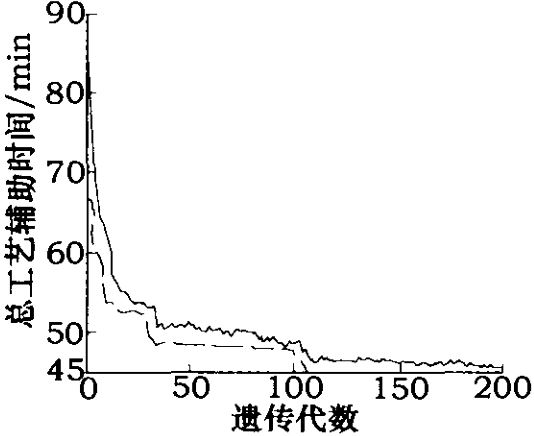
\includegraphics[height = 4.5cm]{AGsimple.jpg}
\caption{遗传算法进化过程\label{fig:AGsimple}}
\end{figure}

设置终止条件为遗传代数不能超过200代,进行了100次的遗传循环过程,采用交叉概率$P_c = 0.80$,变异概率$P_m = 0.08$,得到了最好的生产顺序为:$3\rightarrow12\rightarrow10\rightarrow5\rightarrow6\rightarrow4\rightarrow1\rightarrow8\rightarrow7\rightarrow11\rightarrow2\rightarrow9$,对应的总工艺辅助时间需求为45分钟,其进化过程如\reff{fig:AGsimple}所示。

\subsection{案例小结}
多品种装配调度问题可以看作是典型TSP,虽然具有NP 计算复杂性,但可以通过合理的遗传算法进行求解,找到质量较高的排序方案。在遗传算法的设计中,交叉和变异是跳出局部解的关键,参数的设置需要考虑计算时间和解的质量的权衡。

\section{变邻域搜索在多目标动态调度问题下的运用}
\subsection{背景简述}
在实际生产中,往往需要考虑如机器故障等多种状况,对于调度要求高的地方往往需要考虑众多目标,这使得问题的复杂程度大大增加,简单的搜索算法已经不能适用。变动邻域搜索(VNS)时在区域搜索的基础上,通过扰动,使之跳出区域,以免困于局部最优。所以这个算法包含两个部分,扰动和区域搜索。涉及需要补充概念如下:

\begin{tabular}{ll}
$f$ & 目标函数\\
$S$ & 搜索空间 \\
$x$ & 初始解,$x\in S$\\
$k$ & 寻找最优解的循环中的循环长度控制整数\\
$N_k$ & $(k = 1,2,..,k_{\max})$是扰动和区域搜索函数的相邻结构
\end{tabular}

\subsection{算法步骤对比实验}
通常的作业车间调度模型需要考虑在$m$台机器上完成$n$项作业,需要如下假设:

\begin{asparaitem}
\item 所有机器在同一时刻至多处理一项作业;
\item 所有作业在同一时刻至多被一台机器处理;
\item 处理作业不能被中断;
\item 各项作业的前续作业必须先完成才能进行;
\item 各项作业的工艺路线固定;
\item 作业处理时间和可操作机器事先可知。
\end{asparaitem}
算法具体步骤如下:
\begin{asparaenum}
\renewcommand{\labelenumi}{\heiti 步骤\theenumi~}
\item 选择一个邻域结构$N_k(k\in [1,k_{\max}])$的集合。
\item 设定一个区域搜索的初始解$x$。
\item 选择循环控制量$N$,并设$i=0$。
\item 置$k = 1,\ i = i+1$。
\item 在$x$的第$k$个邻域中随机产生一个节点$x'$。
\item 以$x'$为初始解,并用区域搜索法找到局部近似最优解$x''$。
\item 若$x''$优于$x$,则置$x = x''$,并执行\Step5,否则执行\Step8。
\item 若$k = k_{\max}$则执行\Step9,否则置$k = k+1$并执行\Step5。
\item 若$i\leqslant N$,则执行\Step4,否则算法结束,最优解为$x$。
\end{asparaenum}

\Step1和\Step2为算法的初始化,\Step5为扰动部分,让局部解跳动到邻域,\Step6是区域搜索部分,以找到其中的局部近似最优解,后续步骤皆为循环的控制。\Step6所提到的区域搜索,可用如\reff{fig:local_search}所示的流程来完成。

通过神经网络,学习得到各参数的值,并用最短处理时间(SPT)、先进先出(FIFO)、后进先出(LIFO)、最早工期(EDD)规则作为变邻域搜索的对照,得到计算实验结果如\reff{fig:vnscompare}所示。
\begin{figure}[h]
\centering
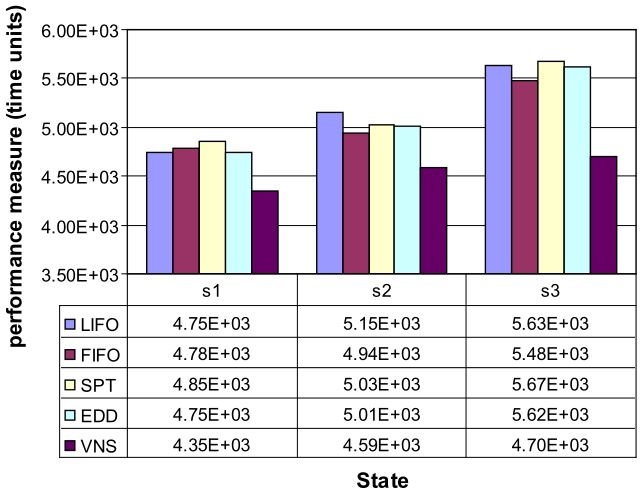
\includegraphics[width = 6cm]{compairsionbasedvns.jpg}
\caption{基于VNS 方法的各调度规则计算结果比较\label{fig:vnscompare}}
\end{figure}
\subsection{案例小结}
变动邻域搜索算法可以应对多目标问题,尤其对动态调度显示出优势,然而其使用的限制还是比较苛刻的,不过其变动策略为求解复杂调度问题提供了新的搜索思路,而且从结果上来看,变动邻域搜索算法的性能很好。